\begin{figure}[H]
        \centerline{
\includegraphics[scale=0.25]{figures/git/git-github-logo}}
        \caption{Git dan Github}
\end{figure}
Seiring berjalannya waktu, setiap pekerjaan manusia selalu mengalami pembaharuan untuk lebih efisien. Tujuannya tidak lain adalah menyederhanakan prosedur pekerjaan yang cenderung berbelit-belit. Begitupun dengan programmer dalam menyusun kode script yang rumit dan panjang membutuhkan kerja tim. Seperti halnya Git dan GitHub muncul untuk membantu pekerjaan tim programmer dalam menyusun kode script. Git dan GitHub merupakan dua platform yang didirikan oleh satu perusahaan dengan tujuan sama serta fitur yang berbeda. Namun kedua platform ini sangat membantu pekerjaan programmer dalam menyusun kode script secara tim. Seluruh pekerjaan juga dapat dipantau dan dievaluasi dengan mudah karena penggunaan kontrol sistem atau bisa disebut Version Control System (VCS). Saat ini, hampir menjadi kewajiban bagi programmer untuk menggunakan kedua platform ini dalam pekerjaannya. Lebih jelasnya, ketahui terlebih dahulu pengertian dari kedua platform berikut ini.


\section{Version Control System (VCS)}
\begin{figure}[H]
        \centerline{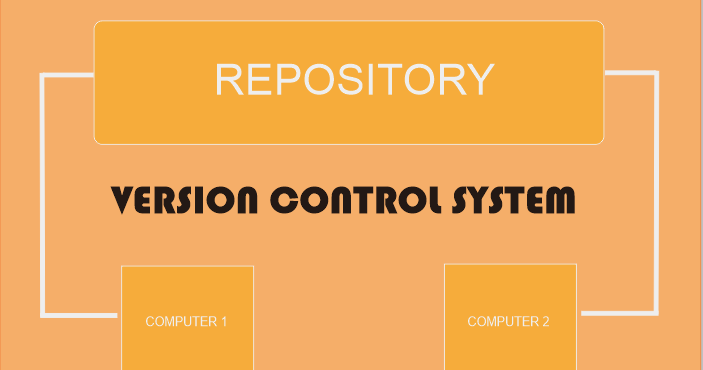
\includegraphics[scale=0.35]{figures/version-control-system/vcs}}
        \caption{Version Control System}
\end{figure}
Version Control System (VCS) adalah sebuah sistem yang melakukan source code management (SCM) )untuk mengelola perubahan di setiap dokumen, program komputer, website, dan kumpulan pemrograman lainnya.
\begin{figure}[H]
        \centerline{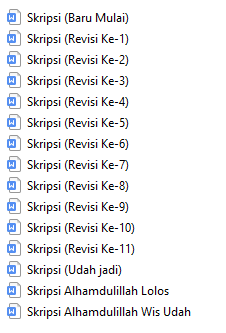
\includegraphics[scale=0.5]{figures/version-control-system/before-vcs}}
        \caption{Sebelum VCS}
\end{figure}
Lebih jelasnya kamu bisa merasakan contoh kasus yang biasa dilakukan oleh seorang mahasiswa dalam mengerjakan skripsinya. Setiap melakukan revisi, file yang telah lalu tidak akan dibuang dan akan disimpan dengan nama yang berbeda. Sedangkan yang terbaru akan disimpan dengan nama; misal “Skripsi (Revisi Ke-2)”. Kegiatan tersebut akan dilakukan secara terus menerus hingga dalam satu folder skripsi terdapat file Ms. Word dengan kuantitas yang banyak. Tujuan tersebut tidak lain adalah untuk menyimpan history pekerjaan mahasiswa. Hingga akhirnya file terakhir selesai dengan nama “Skripsi Alhamdulillah Wis Udah”. Konsep pekerjaan tersebut dianggap tidak efisien oleh banyak developer karena kapasitas penyimpanan akan membengkak. VCS disini berfungsi untuk membantu penyimpanan berupa history tanpa menyimpan file baru, yang tersimpan hanya perubahan data. Sehingga kapasitas penyimpanan file menjadi ringan.
\begin{figure}[H]
        \centerline{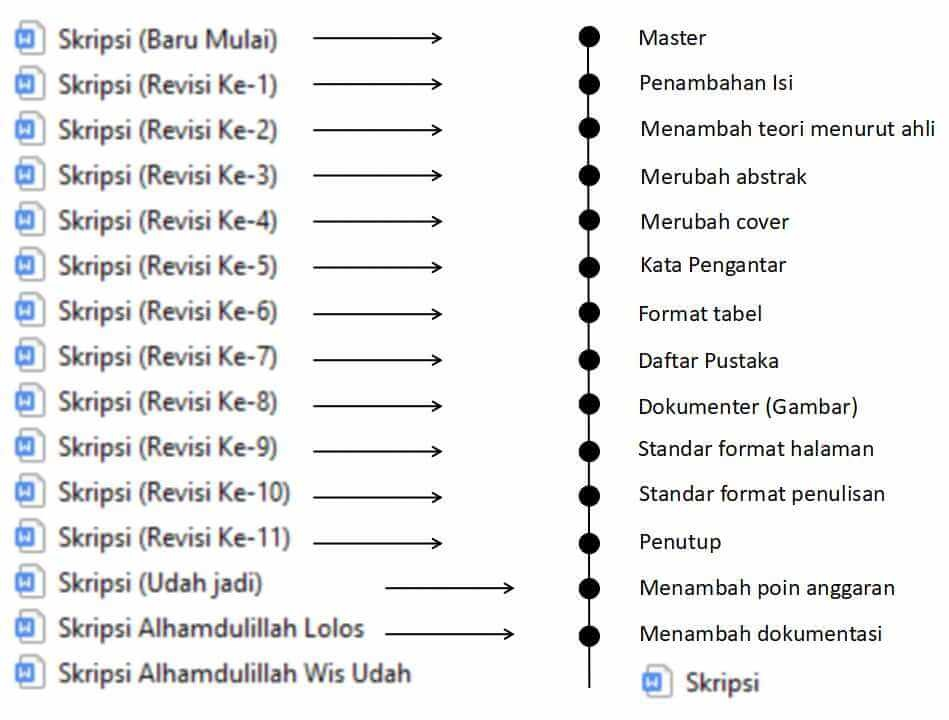
\includegraphics[scale=0.3]{figures/version-control-system/after-vcs}}
        \caption{Sesudah VCS}
\end{figure}
Seperti halnya pada gambar diatas, setiap perubahan data secara manual akan menghasilkan lebih banyak file. Sedangkan pada VCS mengusung konsep menyimpan rekaman perubahan dengan satu file saja.



\section{Git}
\begin{figure}[H]
        \centerline{
\includegraphics[scale=0.15]{figures/git/git-logo}}
        \caption{Git}
\end{figure}
Git merupakan software berbasis Version Control System (VCS) yang bertugas untuk mencatat perubahan seluruh file atau repository suatu project. Developer software biasa menggunakan Git untuk distributed revision (VCS terdistribusi), hal ini bertujuan untuk menyimpan database tidak hanya ke satu tempat. Namun semua orang yang terlibat dalam penyusunan kode dapat menyimpan database ini. Prosedur yang diterapkan ini dapat membantu antar divisi project untuk memantau dan menghubungkan (merge) antar ekstensi yang berbeda dengan mudah. Sehingga aplikasi yang dibuat oleh sebuah tim project dapat berfungsi tanpa menghubungkan secara manual. Terdapat istilah commit pada Git yang berfungsi untuk menyimpan riwayat perubahan data pada file. Melalui commit, developer dapat kembali ke source code sebelumnya dengan istilah checkout. Untuk mengoperasikan Git, kamu perlu menginstall software terlebih dahulu sehingga pekerjaan ini dapat dilakukan secara offline (tidak terkoneksi internet). Software ini juga tersedia secara gratis melalui web unduhan resminya di Git Downloading.


\section{Github}
\begin{figure}[H]
        \centerline{
\includegraphics[scale=0.45]{figures/git/github-logo}}
        \caption{Github}
\end{figure}
GitHub merupakan layanan cloud yang berguna untuk menyimpan dan mengelola sebuah project yang dinamakan repository (repo git). Cara kerja pada GitHub harus terkoneksi pada internet sehingga tidak perlu meng-install sebuah software ke dalam perangkat keras. Hal ini memberikan keringanan penyimpanan komputer yang kita gunakan karena file project tersimpan oleh cloud GitHub. Konsep kerja GitHub pada dasarnya sama dengan Git yaitu dapat menulis source code secara individu atau tim. User interface yang tersedia pada GitHub lebih menarik dan mudah dipahami oleh pengguna awal. Pekerjaan secara tim, pengguna juga bisa melihat siapa penulis kode dan tanggal berapa kode tersebut dibuat. Terdapat fitur lain pada GitHub yaitu kita dapat membaca berbagai blog dan feed yang dibuat oleh sesama pengguna. Hal ini dimanfaatkan oleh pengguna seluruh dunia untuk saling berbagi ide pemrograman dan berdiskusi dalam menyelesaikan masalah. Tentunya postingan yang ada pada GitHub berkaitan dengan pemrograman. Sehingga Github telah menjadi forum diskusi para programmer seperti halnya media sosial. Semenjak GitHub diakuisisi oleh Microsoft di tahun 2018, platform ini berkembang semakin baik dan unggul. Sehingga mayoritas programmer lebih mengenal GitHub dalam program VCS daripada pesaingnya seperti GitLab dan Atlassian BitBucket.


\section{Perbedaan Git \& Github}
Perbedaan antara Git dan GitHub sangat unik dan memiliki keunggulan masing-masing. Berikut ini perbedaan dari kedua platform tersebut.
\begin{center}
\begin{tabular}{ | m{6cm} | m{6cm} | }
\hline
Git & Github \\
\hline
1. Meng-install software di penyimpanan lokal & 1. Host melalui layanan cloud \\
\hline
2. Dikelola oleh The Linux Foundation & 2. Diakuisisi oleh Microsoft pada 2018 \\
\hline
3. Berfokus pada version control dan code sharing & 3. Berfokus pada source code hosting terpusat \\
\hline
4. Akses secara offline & 4. Akses secara online \\
\hline
5. Tidak menggunakan fitur user management & 5. Menggunakan user management \\
\hline
6. Menyediakan desktop interface bernama “Git GUI” & 6. Menggunakan nama desktop interface “GitHub Desktop” \\
\hline
7. Bersaing dengan Mercurial, Subversion, IBM, Rational Team, Concert, dan ClearCase & 7. Bersaing dengan GitLab dan Atlassian BitBucket \\
\hline
8. Open sourced licensed & 8. Pilihan bagi pengguna gratis dan pengguna berbayar \\
\hline
\end{tabular}
\end{center}


\section{Tutorial Membuat Akun Github}
Disini saya akan membahas bagaimana cara mudah membuat akun Github beserta gambar.
\begin{enumerate}
\item kunjungi website \url{https://github.com}, lalu klik sign up untuk mendaftar
\begin{figure}[H]
        \centerline{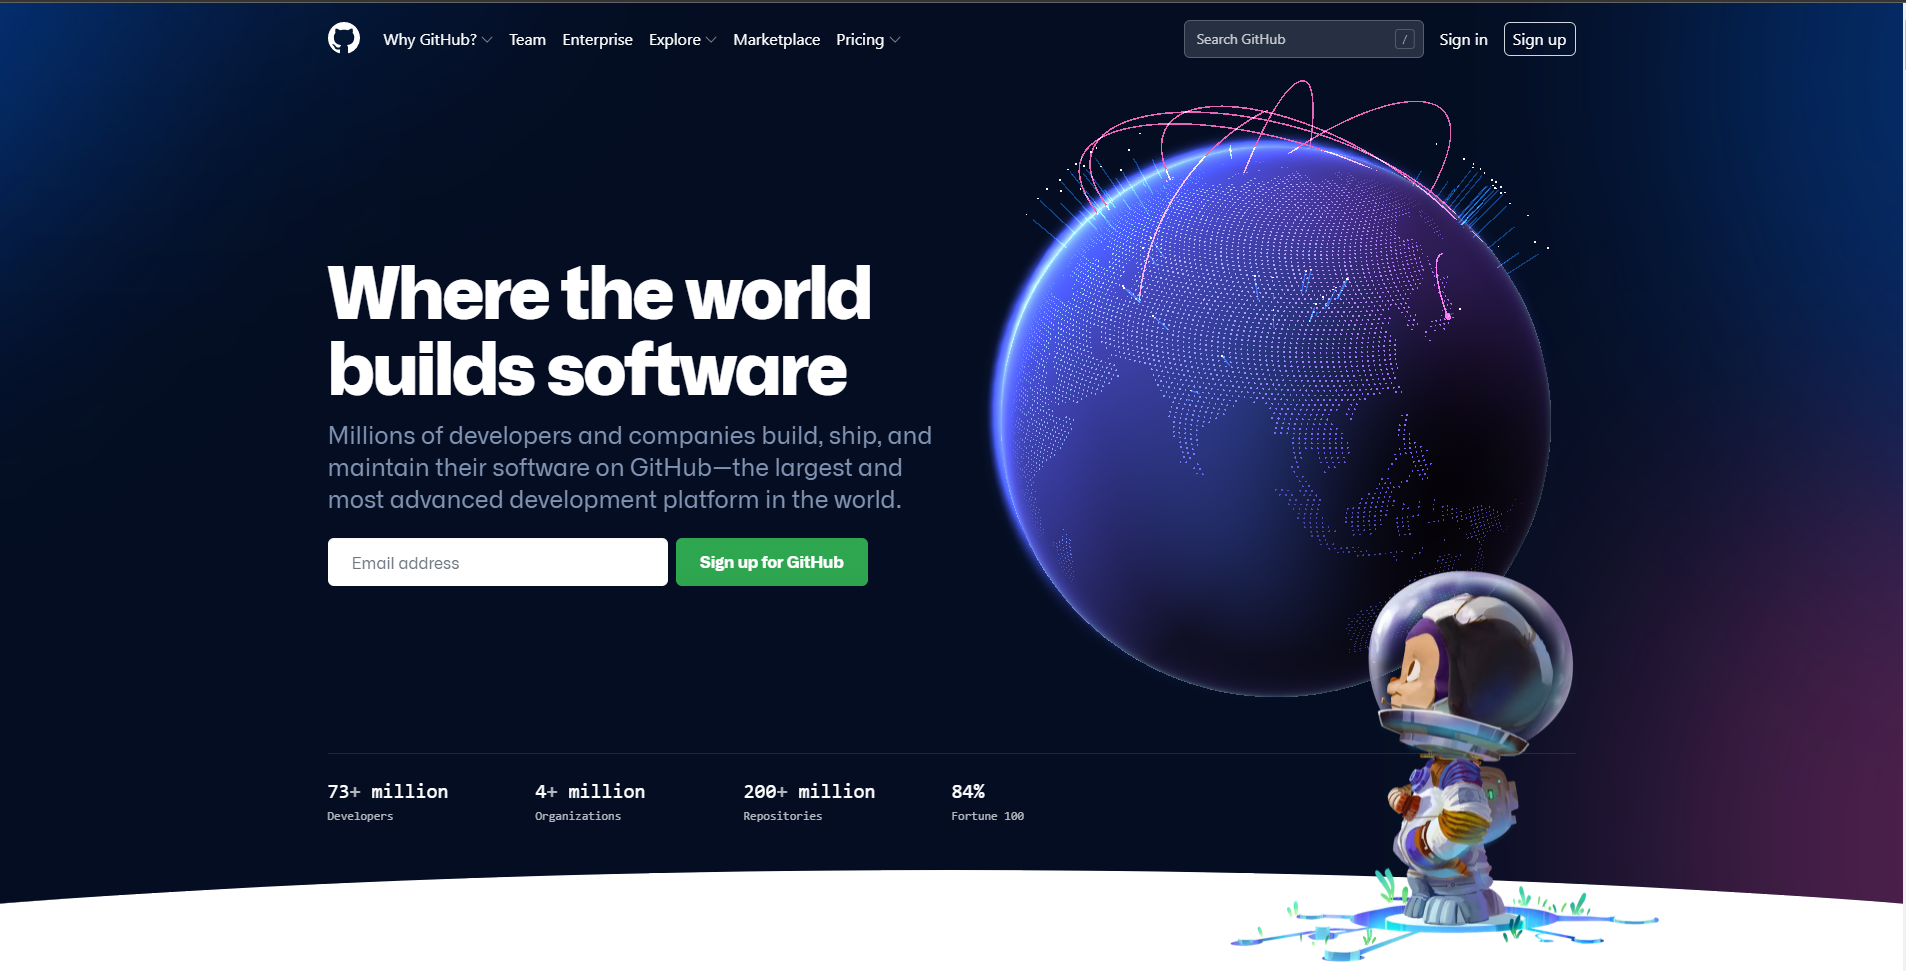
\includegraphics[scale=0.25]{figures/buat-akun-github/step1}}
        \caption{Tutorial Akun Github: Step 1}
\end{figure}
\item lalu akan dialihkan kehalaman pendaftaran, isikan email yang aktif, lalu klik Enter
\begin{figure}[H]
        \centerline{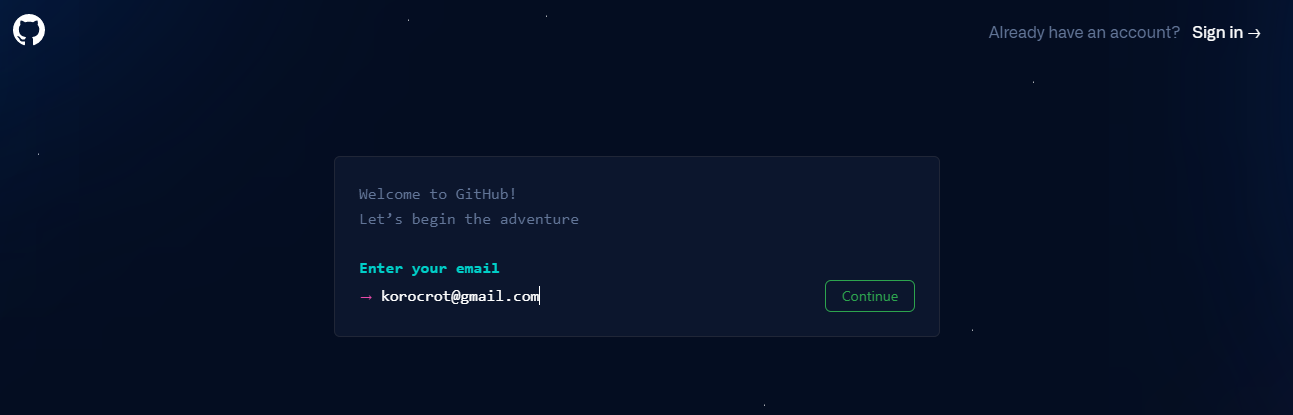
\includegraphics[scale=0.35]{figures/buat-akun-github/step2}}
        \caption{Tutorial Akun Github: Step 2}
\end{figure}
\item lalu masukkan password yang dengan kombinasi yang direkomendasikan oleh Github
\begin{figure}[H]
        \centerline{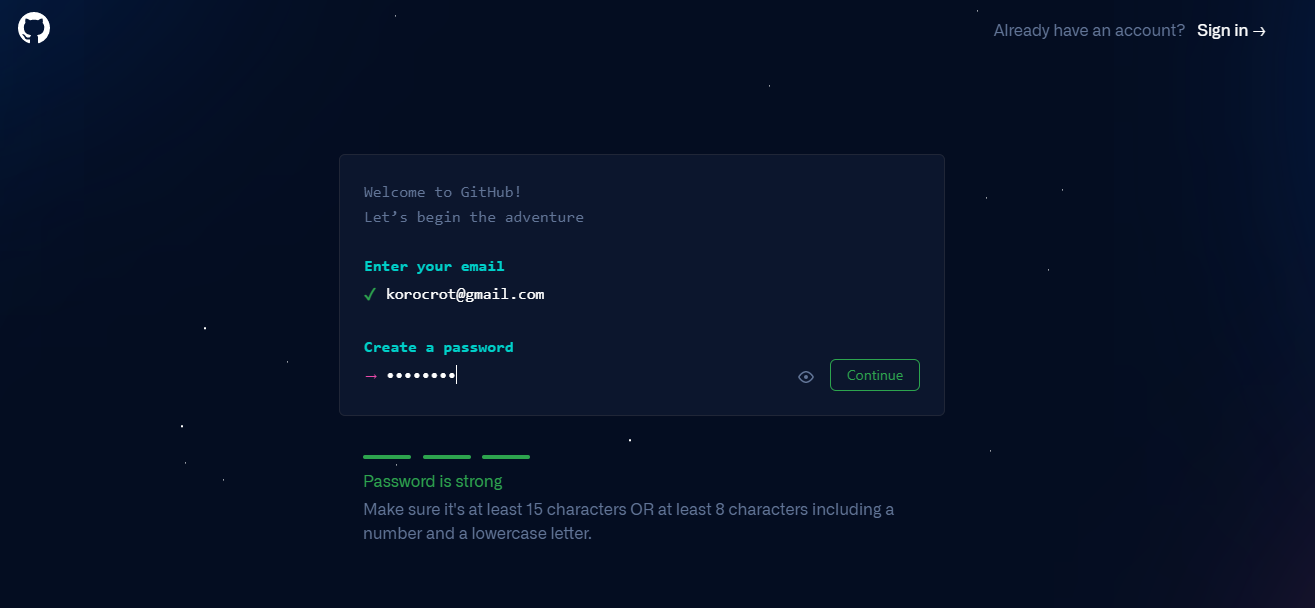
\includegraphics[scale=0.35]{figures/buat-akun-github/step3}}
        \caption{Tutorial Akun Github: Step 3}
\end{figure}
\item masukkan username yang unik, jika username tidak tersedia coba beberapa kombinasi seperti angka dan huruf
\begin{figure}[H]
        \centerline{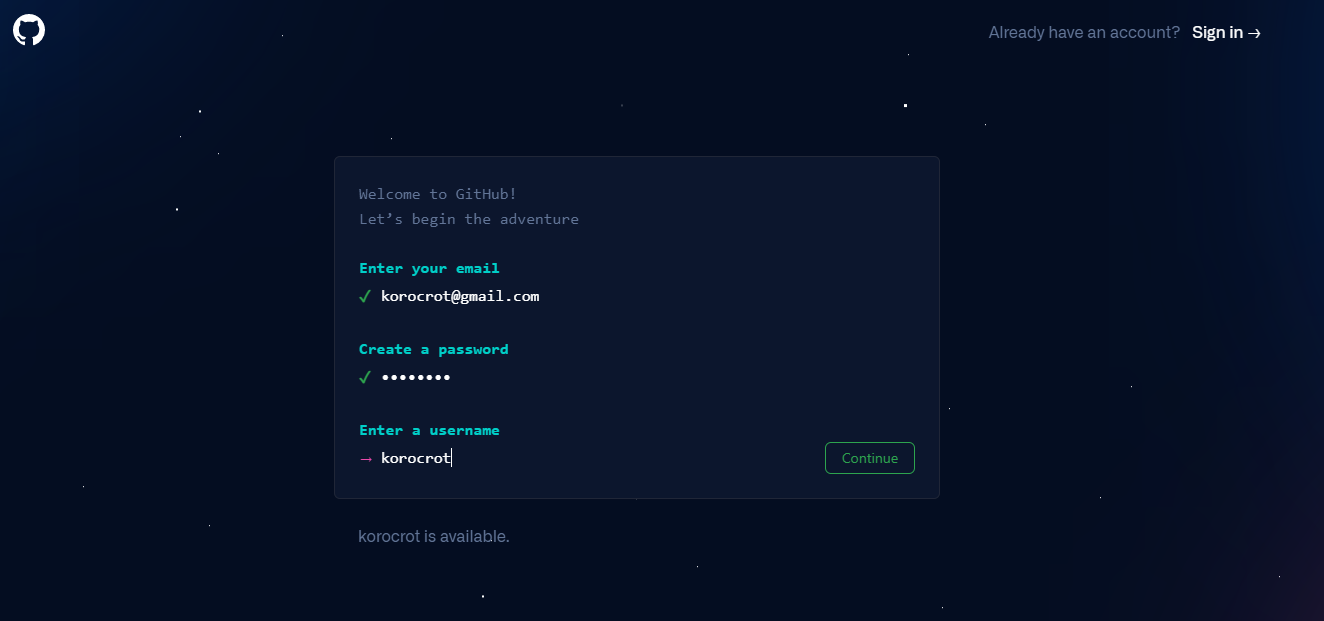
\includegraphics[scale=0.35]{figures/buat-akun-github/step4}}
        \caption{Tutorial Akun Github: Step 4}
\end{figure}
\item lalu setelah itu akan muncul penawaran dari Github untuk notifikasi product dan announcement, saya disini memilih "n"
\begin{figure}[H]
        \centerline{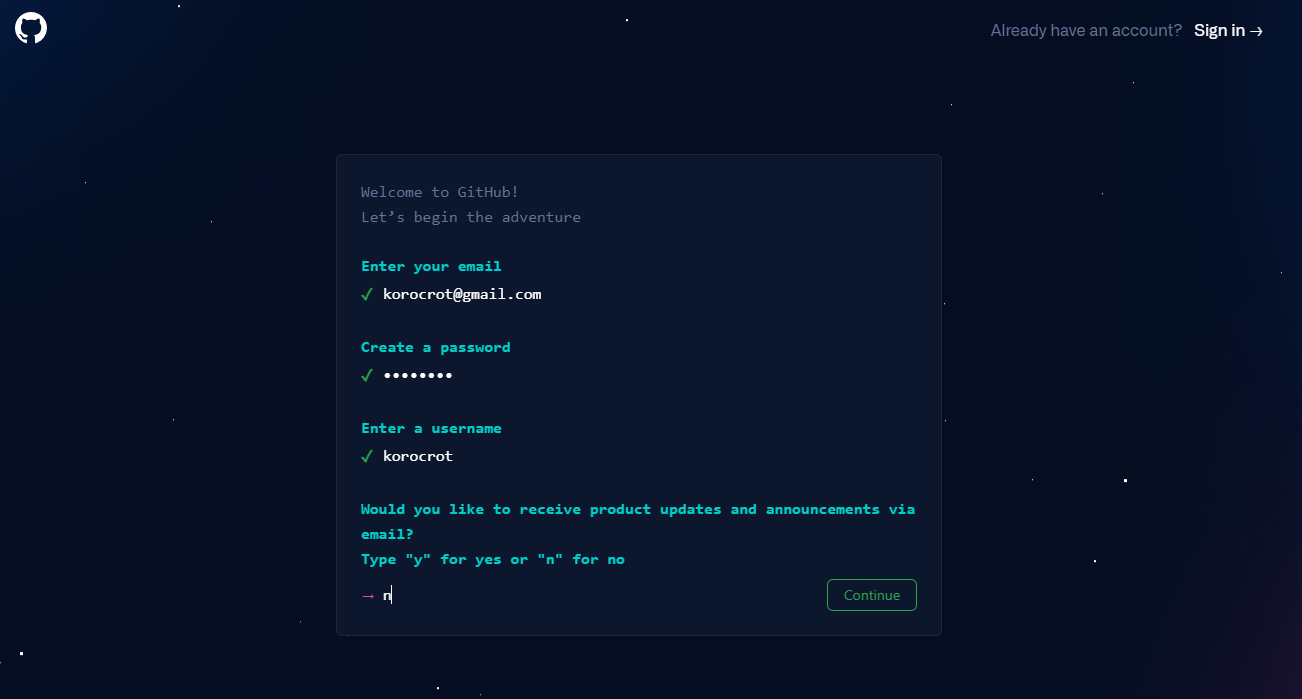
\includegraphics[scale=0.35]{figures/buat-akun-github/step5}}
        \caption{Tutorial Akun Github: Step 5}
\end{figure}
\item setelah itu akan diminta untuk menyelesaikan puzzle untuk verifikasi bahwa yang mendaftar adalah manusia, selesaikan puzze berdasarkan perintah yang diberikan
\begin{figure}[H]
        \centerline{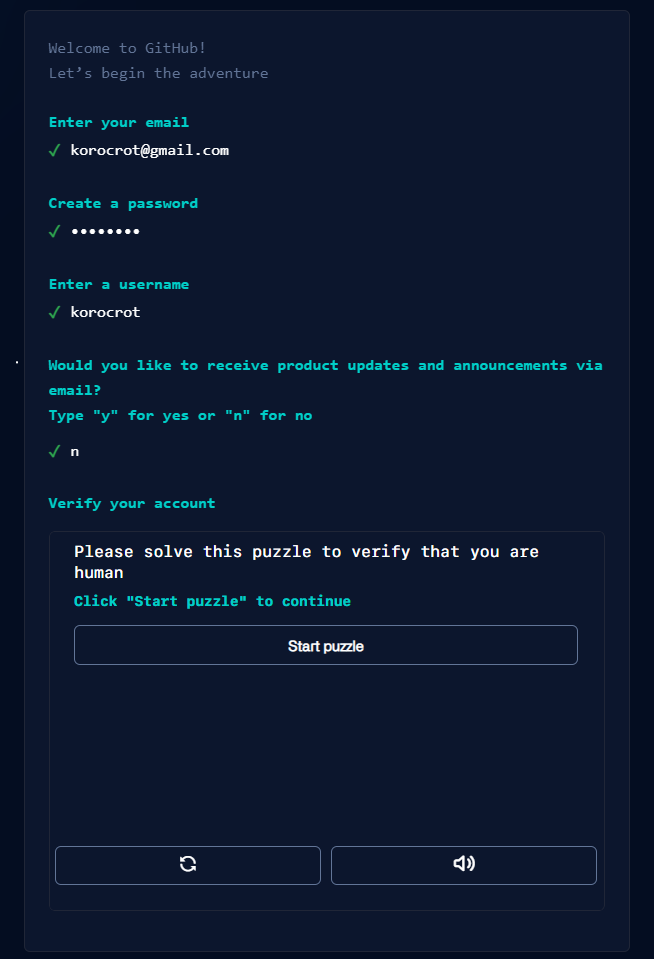
\includegraphics[scale=0.35]{figures/buat-akun-github/step6}}
        \caption{Tutorial Akun Github: Step 6}
\end{figure}
\item jika berhasil bisa langsung klik \textbf{Create account}
\begin{figure}[H]
        \centerline{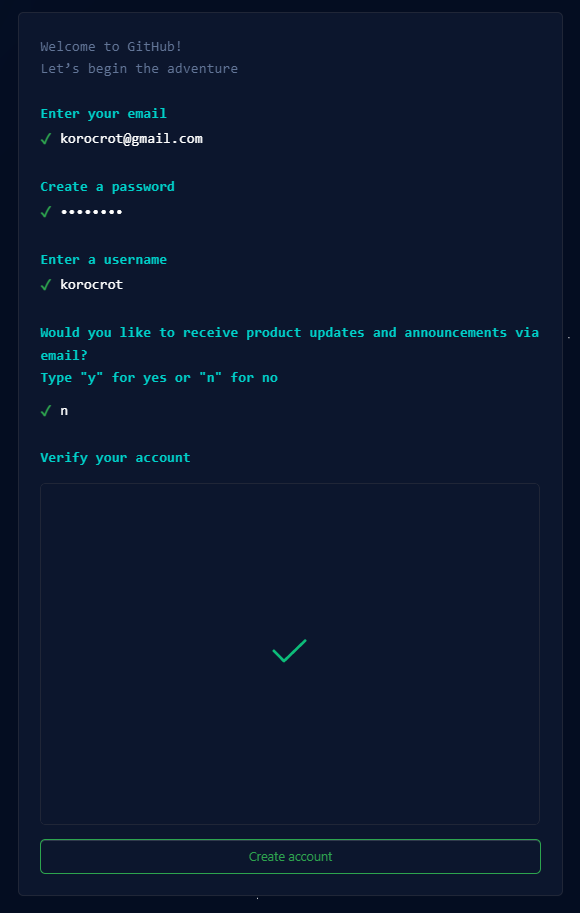
\includegraphics[scale=0.35]{figures/buat-akun-github/step7}}
        \caption{Tutorial Akun Github: Step 7}
\end{figure}
\item lalu Github akan mengirimkan kode verifikasi ke email yang didaftarkan
\begin{figure}[H]
        \centerline{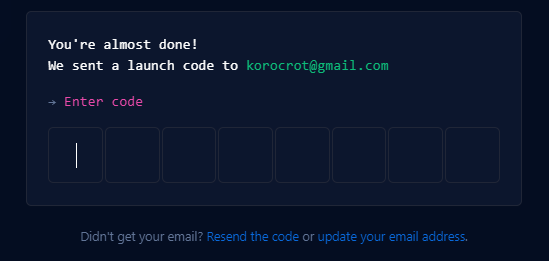
\includegraphics[scale=0.35]{figures/buat-akun-github/step8}}
        \caption{Tutorial Akun Github: Step 8}
\end{figure}
\item copy dan paste code yang ada di email ke kotak \textbf{Enter code} git halaman github, Note: jangan menutup tab Github
\begin{figure}[H]
        \centerline{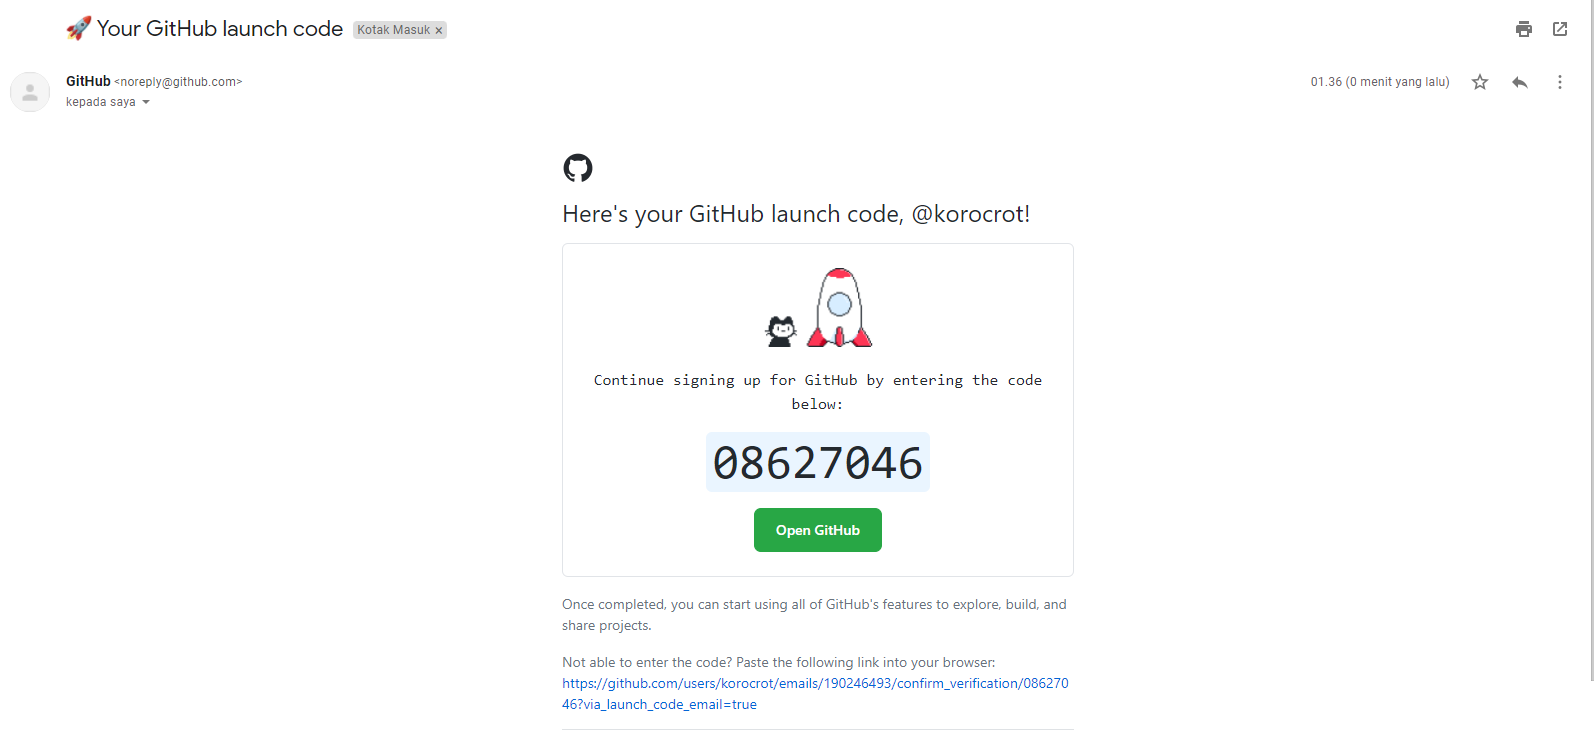
\includegraphics[scale=0.35]{figures/buat-akun-github/step9}}
        \caption{Tutorial Akun Github: Step 9}
\end{figure}
\item jika kode yang dimasukkan benar maka kamu akan dialihkan ke halaman dashboard github
\begin{figure}[H]
        \centerline{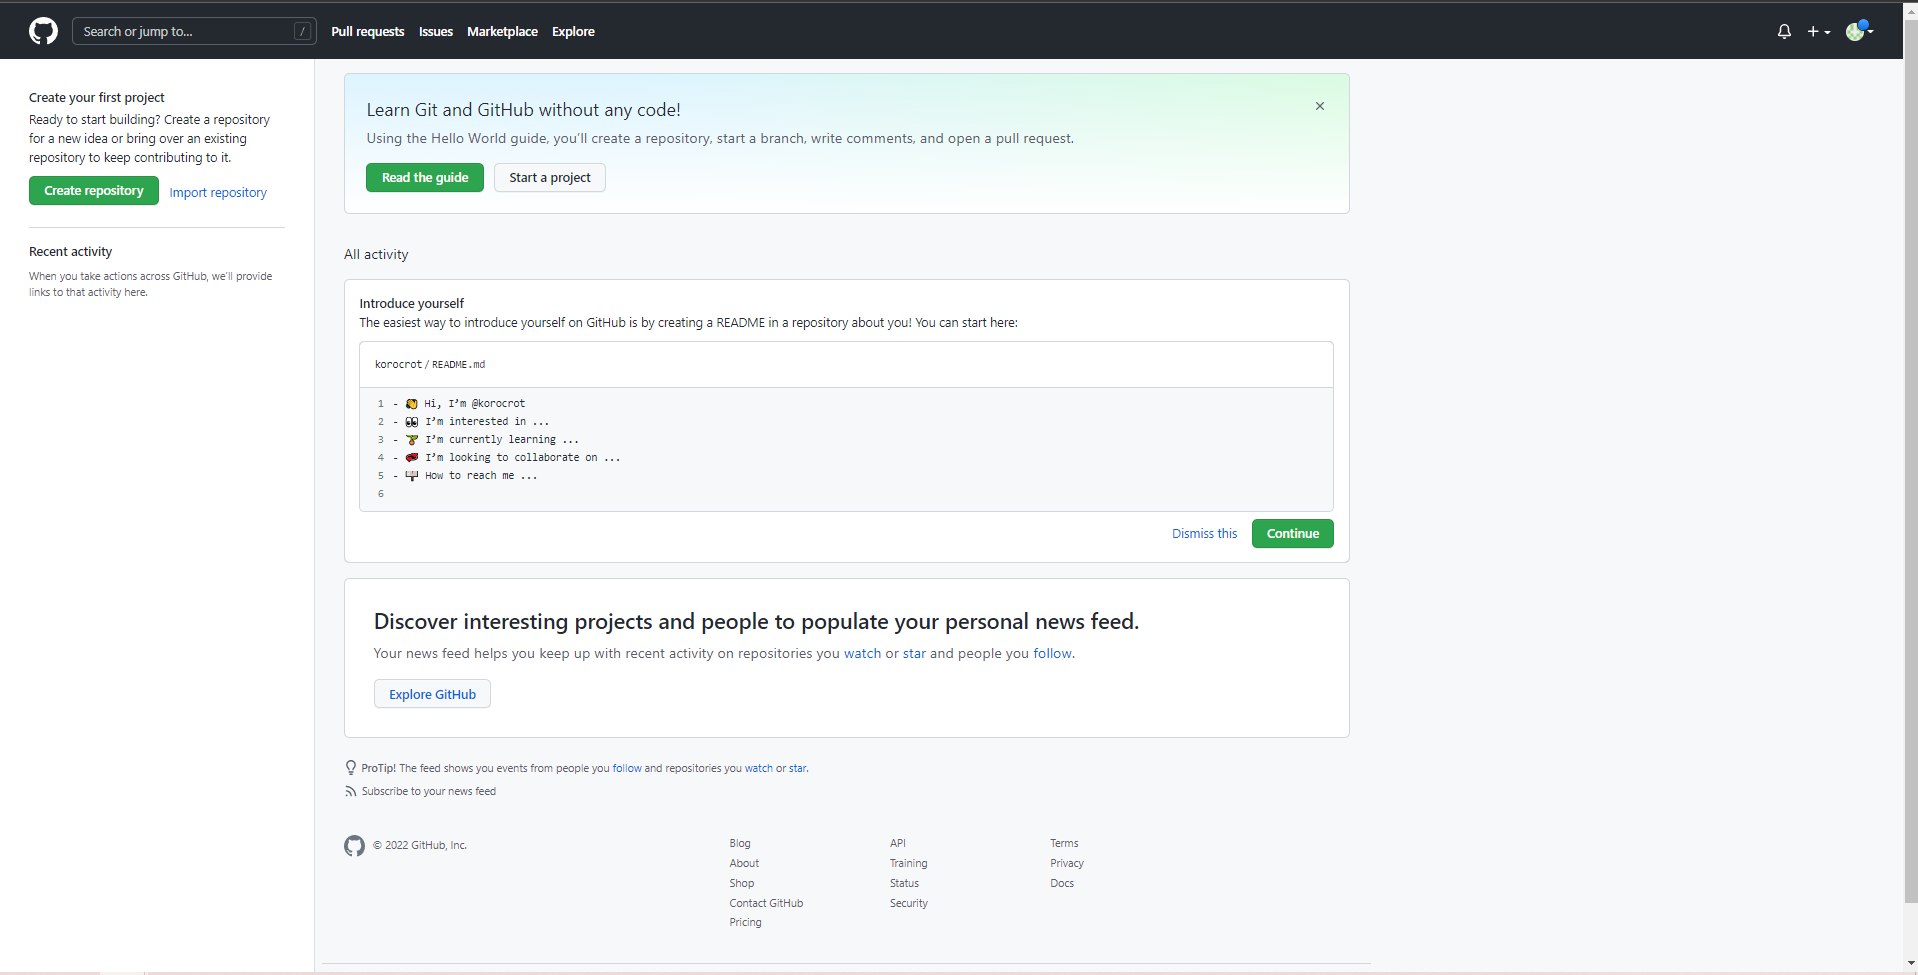
\includegraphics[scale=0.25]{figures/buat-akun-github/step10}}
        \caption{Tutorial Akun Github: Step 10}
\end{figure}
\end{enumerate}


\section{Tutorial Install Git}
Disini saya akan membahas bagaimana cara mudah menginstall Git pada Windows 10 \& Linux beserta gambar.

\subsection{Windows 10}
\begin{enumerate}
\item kunjungi website git-scm \url{https://git-scm.com/}
\item lalu klik menu \textbf{Download}
\item akan muncul seperti gambar dibawah, lalu klik \textbf{Download for Windows}
\begin{figure}[H]
        \centerline{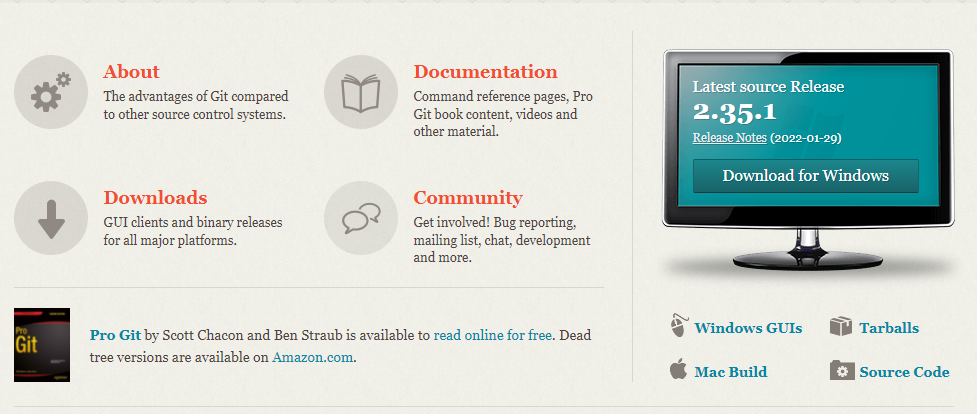
\includegraphics[scale=0.3]{figures/instalasi-git-scm-windows/step1}}
        \caption{Tutorial Install Git-scm: Step 1}
\end{figure}
\item setelah berhasil download, klik (2x) dan akan muncul menu seperti dibawah ini, klik next
\begin{figure}[H]
        \centerline{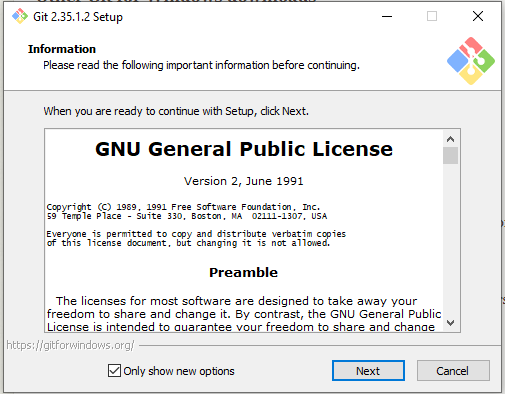
\includegraphics[scale=0.5]{figures/instalasi-git-scm-windows/step2}}
        \caption{Tutorial Install Git-scm: Step 2}
\end{figure}
\item klik next
\begin{figure}[H]
        \centerline{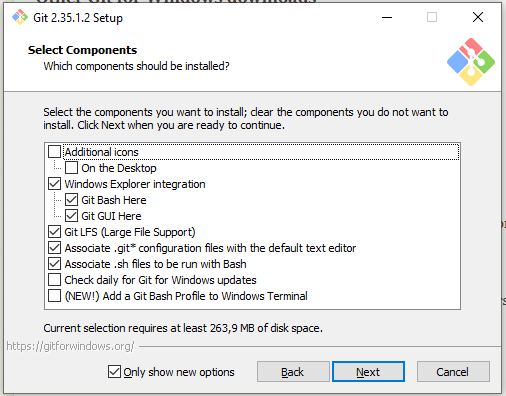
\includegraphics[scale=0.5]{figures/instalasi-git-scm-windows/step3}}
        \caption{Tutorial Install Git-scm: Step 3}
\end{figure}
\item klik next
\begin{figure}[H]
        \centerline{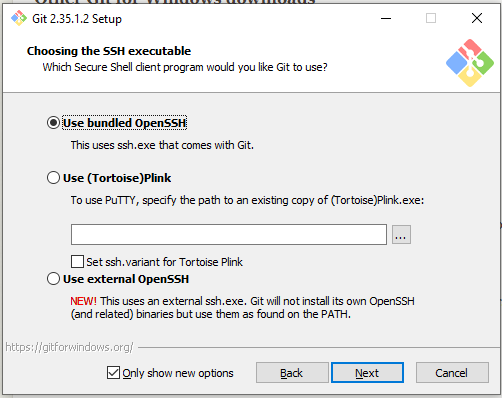
\includegraphics[scale=0.5]{figures/instalasi-git-scm-windows/step4}}
        \caption{Tutorial Install Git-scm: Step 4}
\end{figure}
\item klik install
\begin{figure}[H]
        \centerline{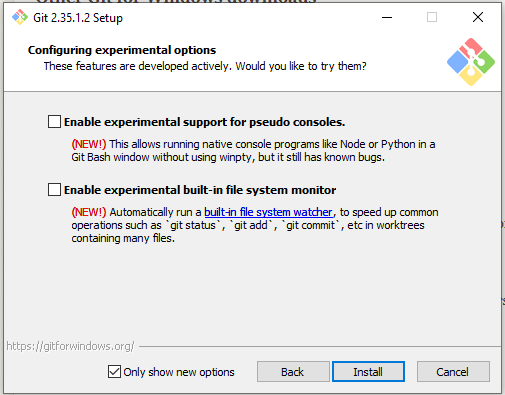
\includegraphics[scale=0.5]{figures/instalasi-git-scm-windows/step5}}
        \caption{Tutorial Install Git-scm: Step 5}
\end{figure}
\item tunggu instalasi hingga selesai
\begin{figure}[H]
        \centerline{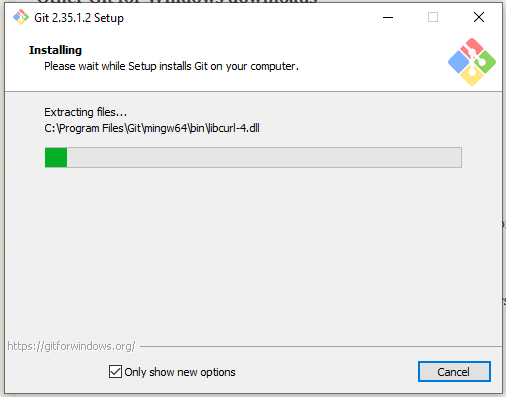
\includegraphics[scale=0.5]{figures/instalasi-git-scm-windows/step6}}
        \caption{Tutorial Install Git-scm: Step 6}
\end{figure}
\item klik finish
\begin{figure}[H]
        \centerline{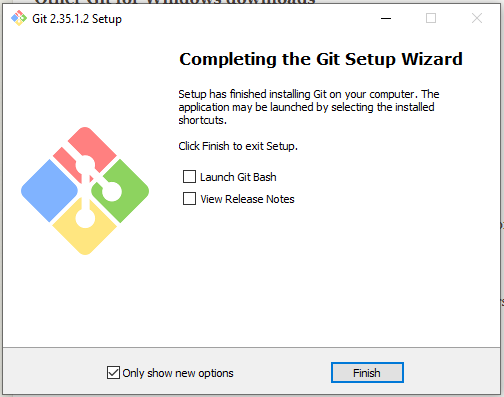
\includegraphics[scale=0.5]{figures/instalasi-git-scm-windows/step7}}
        \caption{Tutorial Install Git-scm: Step 7}
\end{figure}
\end{enumerate}

\subsection{Linux}
untuk instalasi linux bisa dibilang cukup mudah tidak serumit windows, berikut caranya.
\begin{enumerate}
\item buka terminal dan ketikkan \textbf{sudo apt-get install git -y} seperti gambar dibawah ini, lalu tekan Enter
\begin{figure}[H]
        \centerline{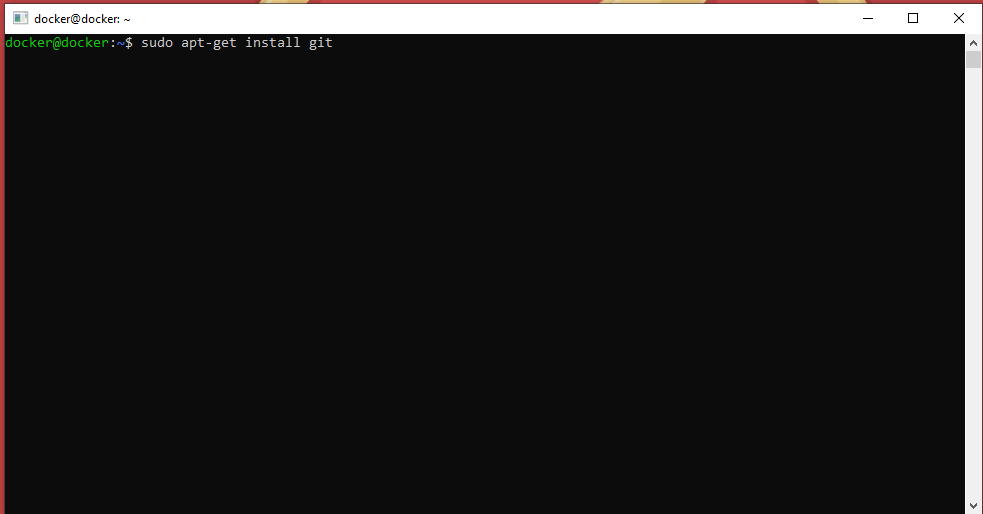
\includegraphics[scale=0.5]{figures/instalasi-git-linux/step1}}
        \caption{Tutorial Install Git Linux: Step 1}
\end{figure}
\item tunggu hingga instalasi selesai seperti gambar dibawah ini
\begin{figure}[H]
        \centerline{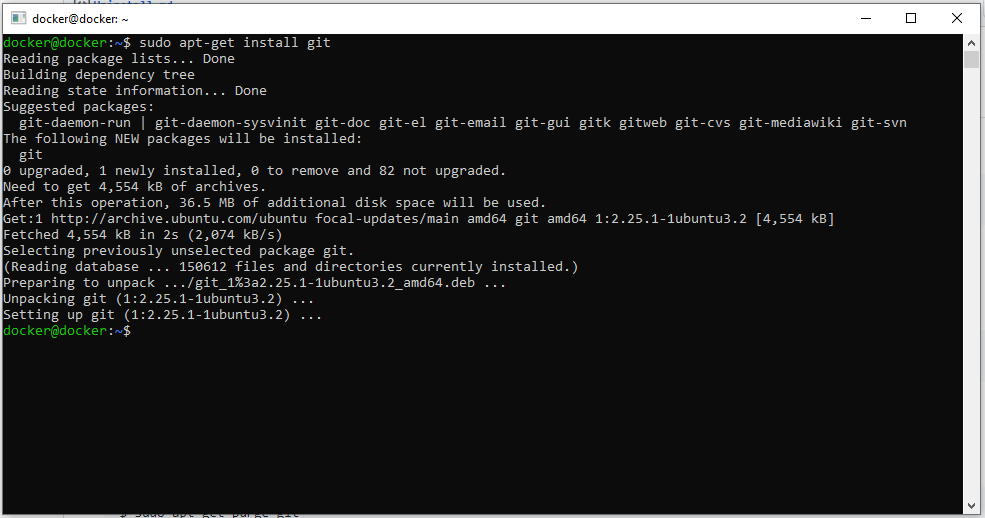
\includegraphics[scale=0.5]{figures/instalasi-git-linux/step2}}
        \caption{Tutorial Install Git Linux: Step 2}
\end{figure}
\end{enumerate}


\section{Generate SSH Key}
Pada section ini saya akan memberikan tutorial cara generate SSH key yang nantinya SSH key tersebut digunakan untuk mengakses website Github.
\begin{enumerate}
\item pertama buka git bash terminal, lalu ketikkan perintah dibawah, lalu tekan Enter
\begin{lstlisting}
ssh-keygen -t rsa -b 4096 -C "email@anda.com"
\end{lstlisting}
\begin{figure}[H]
        \centerline{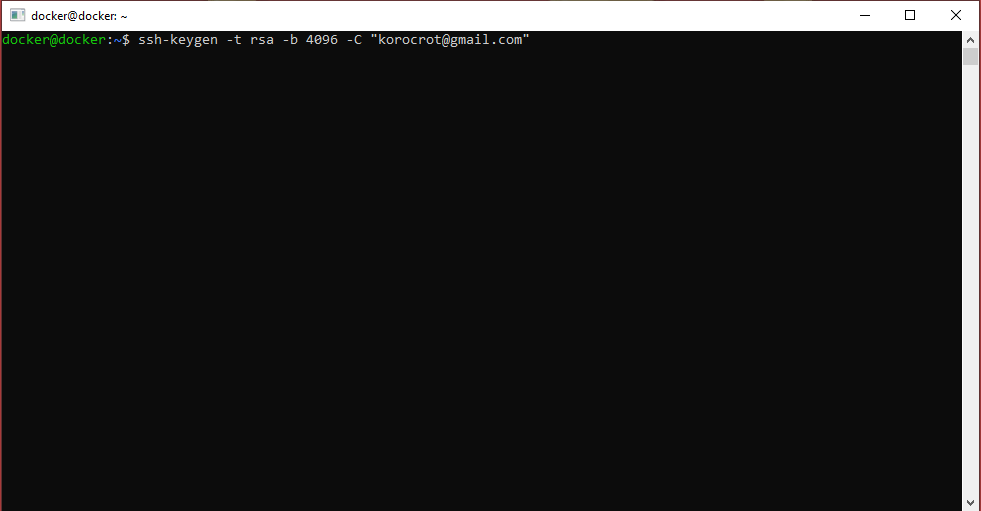
\includegraphics[scale=0.5]{figures/generate-ssh-key/step1}}
        \caption{Tutorial Generate SSH Key: Step 1}
\end{figure}
\item setelah itu akan muncul informasi isian seperti gambar dibawah ini, tekan Enter saja
\begin{figure}[H]
        \centerline{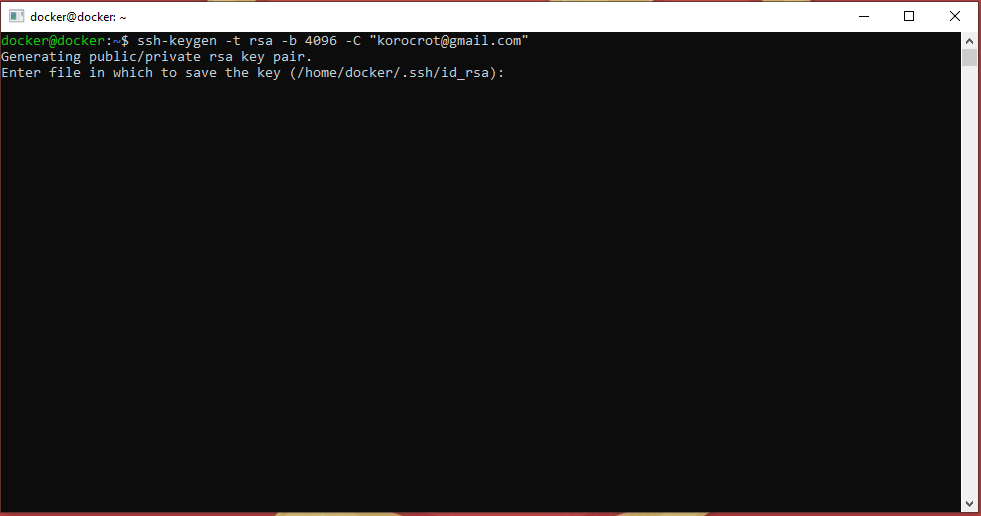
\includegraphics[scale=0.5]{figures/generate-ssh-key/step2}}
        \caption{Tutorial Generate SSH Key: Step 2}
\end{figure}
\item akan muncul lagi isian berikutnya, tekan Enter saja
\begin{figure}[H]
        \centerline{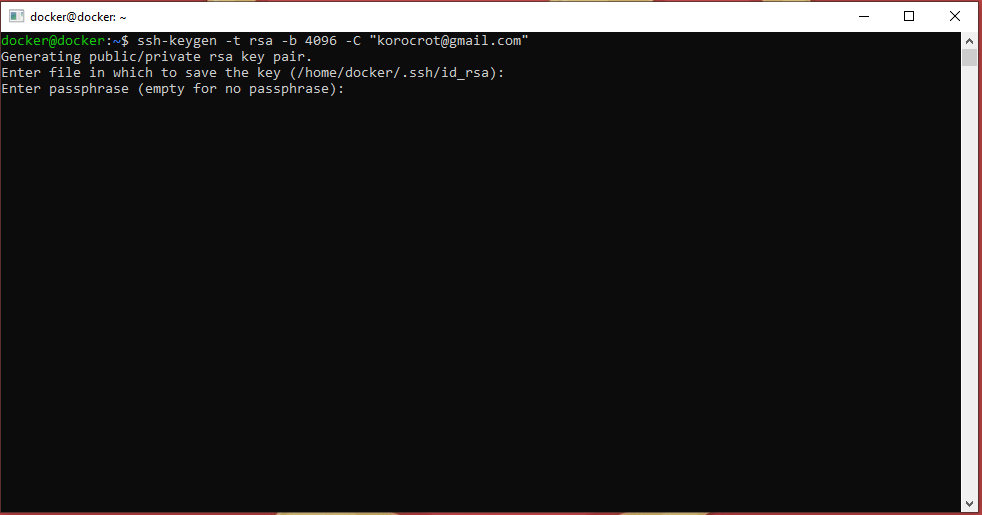
\includegraphics[scale=0.5]{figures/generate-ssh-key/step3}}
        \caption{Tutorial Generate SSH Key: Step 3}
\end{figure}
\item akan muncul lagi isian, tekan Enter saja
\begin{figure}[H]
        \centerline{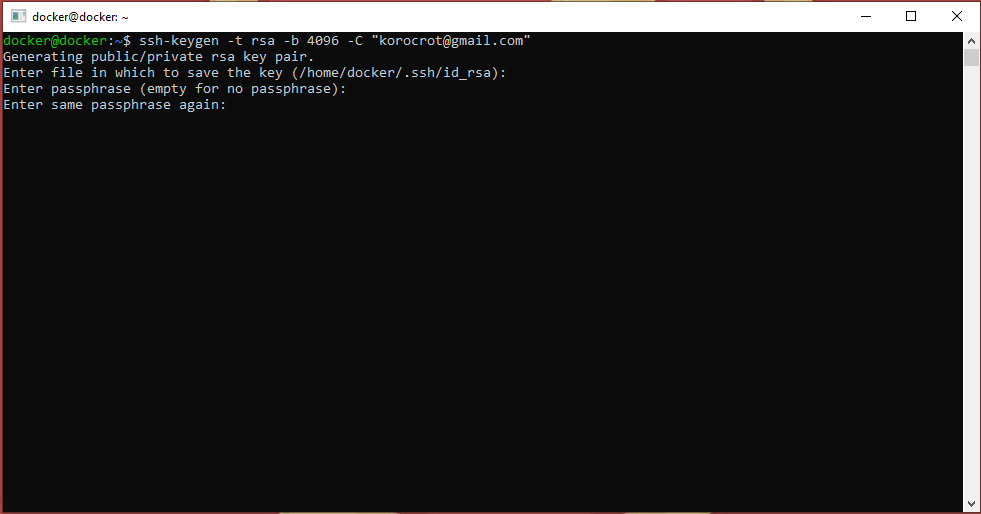
\includegraphics[scale=0.5]{figures/generate-ssh-key/step4}}
        \caption{Tutorial Generate SSH Key: Step 4}
\end{figure}
\item jika sudah selesai akan muncul seperti gambar dibawah ini
\begin{figure}[H]
        \centerline{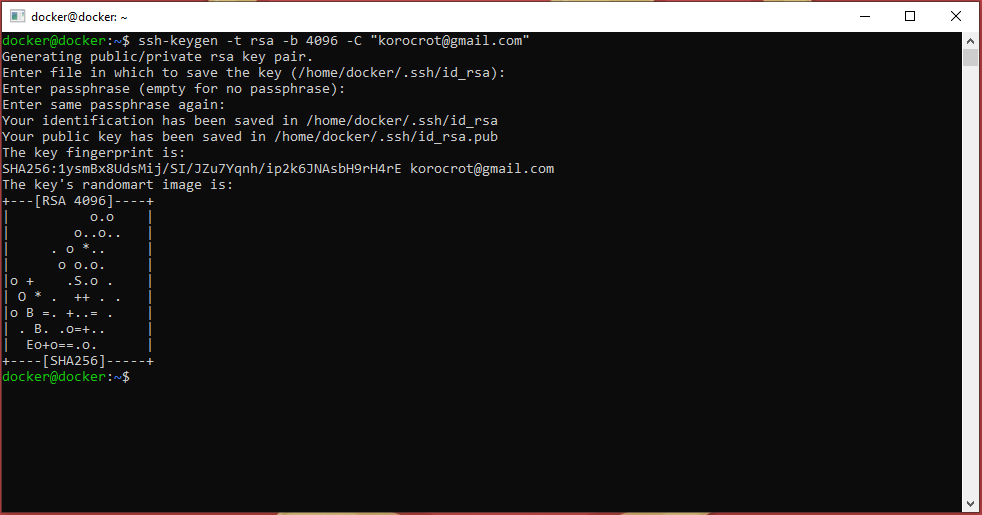
\includegraphics[scale=0.5]{figures/generate-ssh-key/step5}}
        \caption{Tutorial Generate SSH Key: Step 5}
\end{figure}
\end{enumerate}


\section{Memasang SSH Key di Github}
Section ini akan memberikan tutorial bagaimana memasang SSH Key di Github agar komputer bisa terkoneksi dengan akun Github
\begin{enumerate}
\item kunjungi \url{https://github.com} dan login menggunakan akun yang sudah didaftarkan sebelumnya
\begin{figure}[H]
        \centerline{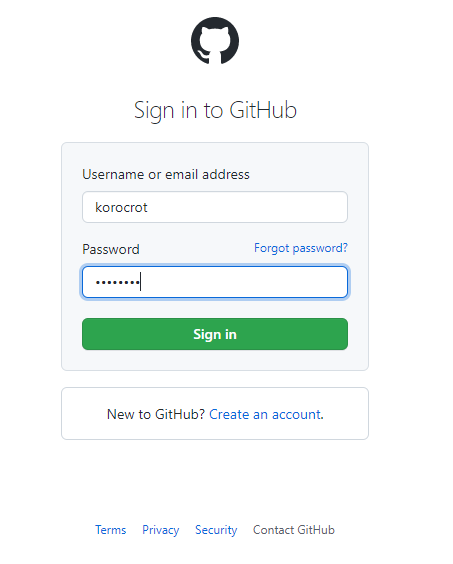
\includegraphics[scale=0.5]{figures/memasang-ssh-key/step1}}
        \caption{Tutorial Memasang SSH Key: Step 1}
\end{figure}
\item jika sudah login klik profile dan klik settings
\begin{figure}[H]
        \centerline{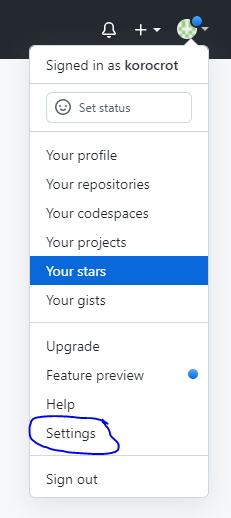
\includegraphics[scale=0.5]{figures/memasang-ssh-key/step2}}
        \caption{Tutorial Memasang SSH Key: Step 2}
\end{figure}
\item setelah itu klik SSH dan GPG Keys
\begin{figure}[H]
        \centerline{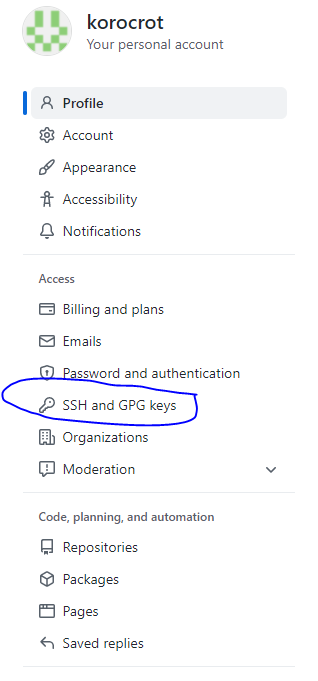
\includegraphics[scale=0.5]{figures/memasang-ssh-key/step3}}
        \caption{Tutorial Memasang SSH Key: Step 3}
\end{figure}
\item lalu klik new ssh keys
\begin{figure}[H]
        \centerline{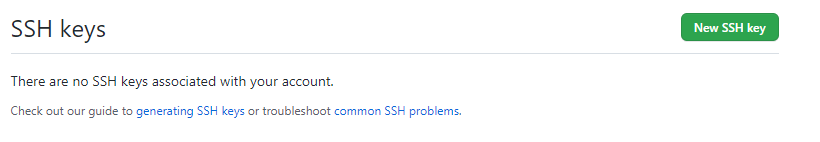
\includegraphics[scale=0.5]{figures/memasang-ssh-key/step4}}
        \caption{Tutorial Memasang SSH Key: Step 4}
\end{figure}
\item lalu buka git bash anda dan ketikkan perintah dibawah, lalu enter, dan copy output yang dikeluarkan
\begin{lstlisting}
cat .ssh/id_rsa.pub
\end{lstlisting}
\begin{figure}[H]
        \centerline{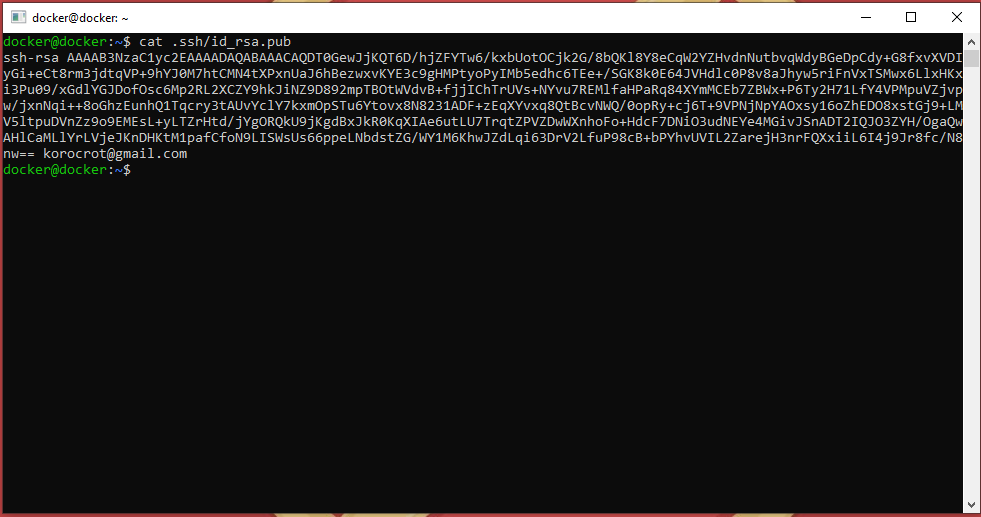
\includegraphics[scale=0.5]{figures/memasang-ssh-key/step5}}
        \caption{Tutorial Memasang SSH Key: Step 5}
\end{figure}
\item setelah itu isi title dengan isian bebas, lalu paste yang sudah dicopy di bagian form bawah seperti gambar dibawah ini, lalu klik add ssh key
\begin{figure}[H]
        \centerline{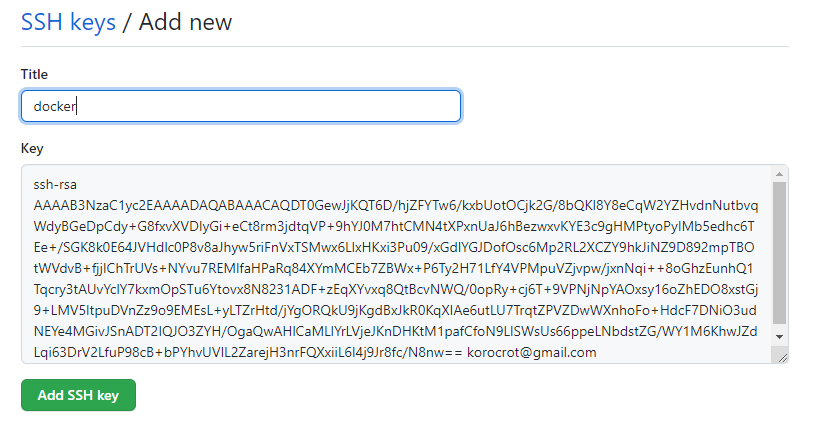
\includegraphics[scale=0.5]{figures/memasang-ssh-key/step6}}
        \caption{Tutorial Memasang SSH Key: Step 6}
\end{figure}
\item jika tampilan seperti dibawah ini maka tahap memasang ssh key sudah selesai
\begin{figure}[H]
        \centerline{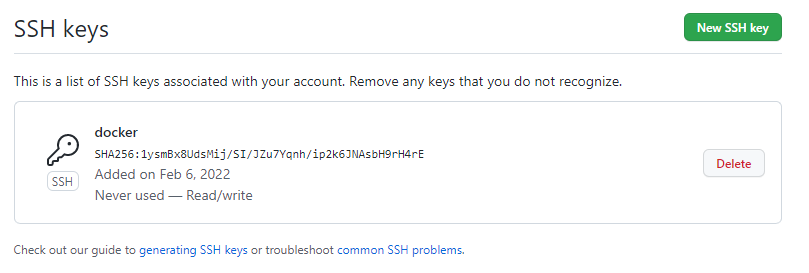
\includegraphics[scale=0.5]{figures/memasang-ssh-key/step7}}
        \caption{Tutorial Memasang SSH Key: Step 7}
\end{figure}
\end{enumerate}
